% Source: Code/camera-to-radar_labeller/system_overview.tex
% Description: Timeline showing radar sweep cadence (1.5s) versus camera observation windows (8--15s). During each camera observation, multiple radar scans occur unobserved by the camera.

\documentclass[border=4pt]{standalone}
\usepackage{amsmath,amssymb,amsfonts}
\usepackage{tikz}
\usepackage{xcolor}
\usetikzlibrary{arrows.meta,positioning,calc,patterns,decorations.markings,shapes.geometric,fit,backgrounds}

\definecolor{Garnet}{HTML}{73000A}
\definecolor{Rose}{HTML}{CC2E40}
\definecolor{Atlantic}{HTML}{466A9F}
\definecolor{Congaree}{HTML}{1F414D}
\definecolor{Horseshoe}{HTML}{65780B}
\definecolor{Grass}{HTML}{CED318}
\definecolor{Honeycomb}{HTML}{A49137}
\definecolor{Black90}{HTML}{363636}
\definecolor{Black70}{HTML}{5C5C5C}
\definecolor{Black50}{HTML}{A2A2A2}
\definecolor{Black30}{HTML}{C7C7C7}
\definecolor{Black10}{HTML}{ECECEC}
\definecolor{WarmGrey}{HTML}{676156}
\definecolor{Sandstorm}{HTML}{FFF2E3}

\tikzset{
    every node/.style={font=\small},
    sysblock/.style={
        draw=Congaree, fill=Congaree!10, thick,
        minimum width=2.2cm, minimum height=1cm,
        align=center, sharp corners,
        text=black
    },
    sysarrow/.style={
        -Stealth, thick, color=Garnet
    },
    timeblock/.style={
        draw=none, fill=#1, minimum height=0.5cm,
        sharp corners, text=white, font=\footnotesize\bfseries,
        inner sep=2pt
    },
    ppiblob/.style={
        fill=#1, sharp corners, minimum size=4pt, inner sep=0pt
    },
}

\begin{document}
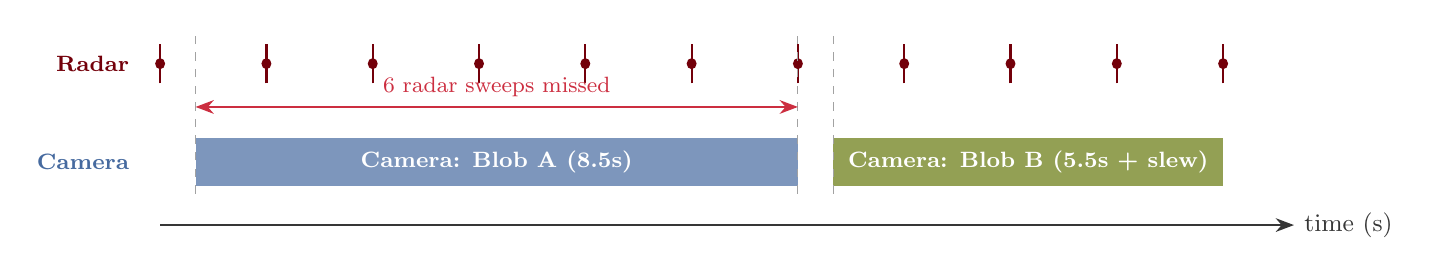
\begin{tikzpicture}[xscale=0.9]
    % Time axis
    \draw[-Stealth, thick, color=Black90] (0,0) -- (16,0) node[right] {time (s)};

    % Radar sweeps
    \foreach \i in {0,1.5,...,15} {
        \draw[thick, Garnet] (\i, 1.8) -- (\i, 2.3);
        \fill[Garnet] (\i, 2.05) circle (2pt);
    }
    \node[left, font=\footnotesize\bfseries, text=Garnet] at (-0.3, 2.05) {Radar};

    % Camera windows
    \fill[Atlantic, opacity=0.7] (0.5, 0.5) rectangle (9.0, 1.1);
    \node[font=\footnotesize\bfseries, text=white] at (4.75, 0.8) {Camera: Blob A (8.5s)};

    \fill[Horseshoe, opacity=0.7] (9.5, 0.5) rectangle (15.0, 1.1);
    \node[font=\footnotesize\bfseries, text=white] at (12.25, 0.8) {Camera: Blob B (5.5s + slew)};

    \node[left, font=\footnotesize\bfseries, text=Atlantic] at (-0.3, 0.8) {Camera};

    % Annotations
    \draw[Black50, dashed] (0.5, 0.4) -- (0.5, 2.5);
    \draw[Black50, dashed] (9.0, 0.4) -- (9.0, 2.5);
    \draw[Black50, dashed] (9.5, 0.4) -- (9.5, 2.5);

    % Sweep count annotation
    \draw[Stealth-Stealth, Rose, thick] (0.5, 1.5) -- (9.0, 1.5)
        node[midway, above, font=\footnotesize, text=Rose] {6 radar sweeps missed};
\end{tikzpicture}
\end{document}
